\section{Auswertung}
	\label{sec:Auswertung}

	\subsection{Bestimmung des Dunkelstroms}
		\label{sub:bestimmung_des_dunkelstroms}
		
		Um die Messwerte mit der Theorie vergleichen zu k"onnen muss zuerst der Dunkelstrom $I_\mathrm{du}$ gemessen werden.

		Dazu wurde unter Versuchsbedingungen, jedoch mit ausgeschaltetem Laser, eine Messung durchgef"uhrt.

		F"ur den Dunkelstrom ergab sich:

		\begin{equation}
			I_\mathrm{du} = \SI{0.13}{\nano \ampere}
		\end{equation}

		Die Aufgetragenenen Messwerte in den Tabellen sind noch nicht um diesen Wert reduziert.

	\subsection{Bestimmung der Spaltbreite eines festen Einfachspalts}
		\label{sub:bestimmung_der_spaltbreite_eines_festen_einfachspalts}
		
		Im folgenden wird die Spaltbreite eines Einfachspalts auf zwei verschiedene Weisen gemessen. Einmal mithilfe des Beugungsmusters und einmal mit Hilfe eines Mikroskops.

		\subsubsection{Bestimmung mit Hilfe des Beugungsmusters}
			\label{sub:Bestimmung_mit_Hilfe_des_Beugungsmusters}

			Wie die Spaltbreite bestimmt wird, wird bereits in \ref{sec:messung} erl"autert. Die bereinigten Messwerte finden sich in Tabelle \ref{tabelle_1} wieder.

			Die gemessene Intensit"at wurde in Grafik \ref{graf_1} gegen die Detektorposition aufgetragen und eine Theoriekurve nach Gleichung \ref{prop_einzelspalt} eingef"ugt um die Kurven vergleichen zu k"onnen.

			Zur Anpassung wurde Gnuplot benutzt.

			Es ergibt sich mithilfe der Formel:

			\begin{equation}
				f(x) = a^2 b^2 \left(\frac{\lambda}{\pi b \sin(\frac{x-x_\mathrm{0}}{d})}\right)^2 \sin^2 \left( \frac{\pi b \sin(\frac{x-x_\mathrm{0}}{d})}{\lambda} \right)
			\end{equation}

			der Wert:

			\begin{equation}
				b = \SI{74.6 (17)}{\micro \meter}
			\end{equation}

			\begin{table}[h]
\begin{center}
\begin{tabular}{c|c|c||c|c|c||c|c|c}
Ub[V] & Ud[V] & D[1/4 in] & Ub[V] & Ud[V] & D[1/4 in] & Ub[V] & Ud[V] & D[1/4 in] \\
\hline
200 & -7,1 & 4 & 250 & -9,3 & 4 & 300 & -11,9 & 4 \\
200 & -3,9 & 3 & 250 & -5,2 & 3 & 300 & -7,1 & 3 \\
200 & -0,1 & 2 & 250 & -0,4 & 2 & 300 & -1,2 & 2 \\
200 & 3,4 & 1 & 250 & 4 & 1 & 300 & 4,3 & 1 \\
200 & 6,9 & 0 & 250 & 8,4 & 0 & 300 & 9,5 & 0 \\
200 & 10,5 & -1 & 250 & 12,6 & -1 & 300 & 14,8 & -1 \\
200 & 13,7 & -2 & 250 & 17,3 & -2 & 300 & 20,4 & -2 \\
200 & 17,4 & -3 & 250 & 21,4 & -3 & 300 & 25,3 & -3 \\
200 & 20,7 & -4 & 250 & 25,4 & -4 & 300 & 30,0 & -4 \\
\end{tabular}
\caption{Messwerte zu Aufgabe a bei verschiedenen Beschleunigungsspannungen}
\label{tabelle_1}
\end{center}
\end{table}

			\begin{figure}[H]
				\centering
				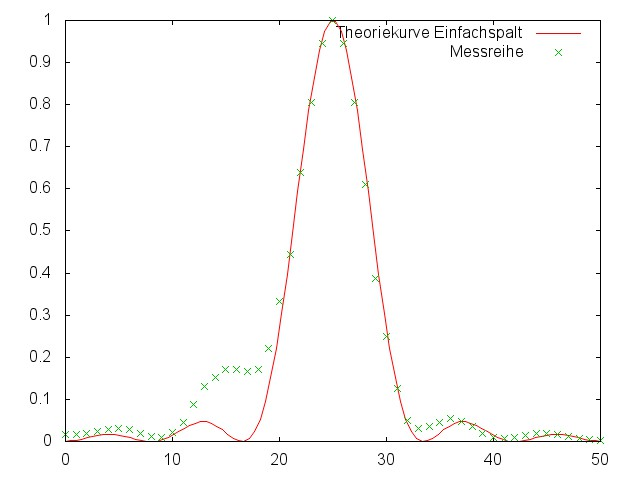
\includegraphics[width = 14cm]{graph1.jpg}
				\caption{Graphische Darstellung der Beugung eines festen Einfachspalt}
				\label{graph1}
			\end{figure}

			Die errechnete Spaltbreite $b$ entspricht nicht exakt der vorgegebenen von $b = \SI{80}{\micro \meter}$, ist aber gr"o"sentechnisch nicht weit davon weg.

			Auf m"ogliche Fehlerquellen wird in der Diskussion eingegangen.
			\newpage

		\subsubsection{Bestimmung mit Hilfe des Mikroskops}
			\label{sub:Bestimmung_mit_Hilfe_des_mikroskops}

			Das Ausmessen mithilfe des Mikroskops wurde bereits in \ref{sec:messung_mikro} erkl"art.
			Es wurde auf das Objektmikrometer fokussiert. Nun wurde der Spalt unter das Objektiv gelegt und mithilfe eines verschiebbaren Teilstrichs die Spaltkanten "uberdeckt. Diese Fixierung wurde dann auf die Mikrometerskala des Objektmikrometers gelegt und ausgemessen.
			Aufgrund von Unsch"arfen wurde ein Fehler von $\sigma_0 = \SI{10}{\micro \meter}$ angenommen.

			Es ergab sich f"ur die Spaltbreite b:

			\begin{equation}
				b = \SI{70}{\micro \meter}
			\end{equation}

			Damit ergibt sich f"ur die gemessene Spaltbreite $b_\mathrm{mikro} = \SI{70 (10)}{\micro \meter}$.
			Es besteht ein gro"ser Unterschied zwischen der gemessenen und der angegebenen Spaltbreite von $b = \SI{80}{\micro \meter}$.
			Auf Fehlerquellen wird in der Diskussion eingegangen.
			\clearpage
			\newpage

	\subsection{Bestimmung der Spaltbreite eines variablen Einfachspalts} 
		\label{sub:bestimmung_der_spaltbreite_eines_variablen_einfachspalts}
		
		Nun sollte die Breite $b$ eines variablen Einfachspalts gemessen werden. Das Messverfahren ist dasselbe wie zuvor.

		Die dazugeh"origen Intensit"atswerte abh"angig von der Detektorposition finden sich in Tabelle \ref{tabelle_2}. Weiter wurde eine Theoriekurve in die Grafik \ref{graph1} einge"ugt, sodass ein Vergleich zwischen Theorie und Experiment m"oglich ist. Daf"ur wurde Gnuplot verwendet.

		Es ergab sich:

		\begin{equation}
			b = \SI{100.0 (23)}{\micro \meter}
		\end{equation}

		\begin{table}[h]	
\centering
\begin{tabular}{|l l||l l||l l|} \hline
	x[mm] & I[nA] & x[mm] & I[nA] & x[mm] & I[nA]\\
	\hline
	0	&	2.5   &  17	&	15  & 34	&	4.8\\
	1	&	2.1   &  18	&	13  & 35	&	3\\
	2	&	2.1   &  19	&	12.5& 36	&	1.85\\
	3	&	2.5   &  20	&	23.5& 37	&	1.55\\
	4	&	2.9   &  21	&	50  & 38	&	2.1 \\
	5	&	2.85  &  22	&	98  & 39	&	2.85\\
	6	&	2.5   &  23	&	135 & 40	&	3\\
	7	&	2.75  &  24	&	165 & 41	&	2.8\\
	8	&	4     &  25	&	155 & 42	&	1.95\\
	9	&	6.2   &  26	&	125 & 43	&	1\\
	10	&	8     &  27	&	92  & 44	&	0.6\\
	11	&	7.9   &  28	&	50  & 45	&	0.51\\
	12	&	6     &  29	&	25.5& 46	&	0.72\\
	13	&	4     &  30	&	11  & 47	&	0.86\\
	14	&	4.8   &  31	&	7.2 & 48	&	0.86\\
	15	&	8.5   &  32	&	6.4 & 49	&	0.68\\
	16	&	13    &  33	&	6   & 50	&	0.45\\
	\hline
\end{tabular}
\caption{Intensit"at des festen Einfachspalts abgh"angig von der Detektorstellung x}
\label{tabelle_2}
\end{table}



		\begin{figure}[H]
			\centering
			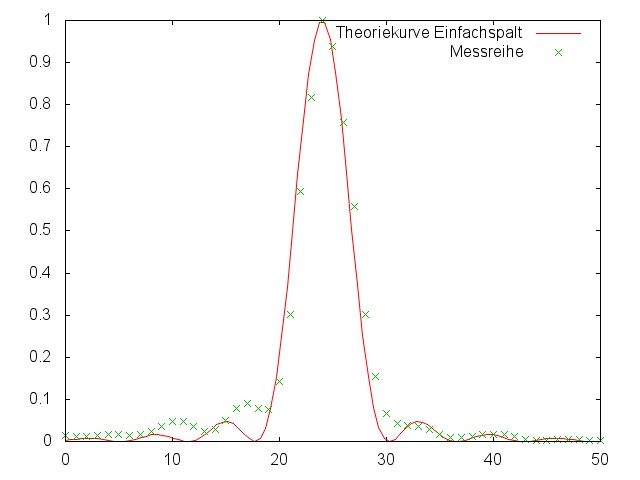
\includegraphics[width = 14cm]{graph2.jpg}
			\caption{Graphische Darstellung der Beugung eines variablen Einfachspalt}
			\label{graph2}
		\end{figure}

		F"ur die Spaltbreite $b$ hat sich in der Messung ein Wert innerhalb des Bereiches von $20-200 \SI{}{\micro \meter}$ ergeben. Da es sich um einen variablen Einfachspalt mit unbekannter Gr"o"se handelt, kann nicht genau gesagt werden wie weit vom tats"achlichen Wert abgewichen wurde. Es ist jedoch mit einem Fehler zu rechnen.

\clearpage
		\newpage
		\newpage
	\subsection{Bestimmung der Spaltbreite eines festen Doppelspalts} 
	\label{sub:bestimmung_der_spaltbreite_eines_festen_doppelspalts}
	
		Auch hier wurde dasselbe Verfahren wie bei den vorherigen Messungen angewendet.
		Die Messwerte sind in Tabelle \ref{tabelle_3} zu finden und der dazugeh"orige Graph mit Theorikurve nach Gleichung \ref{prop_doppelspalt} in Grafik \ref{graph3}.

		F"ur die Spaltbreite $b$ und den Abstand zwischen den Spalten $d$ ergab sich:

		\begin{eqnarray*}
			b &=& \SI{33.5 (16)}{\micro \meter}\\
			d &=& \SI{226.7 (23)}{\micro \meter}
		\end{eqnarray*}

		Die gemessenen Werte weichen abermals nicht sehr von den ablesbaren Werten auf der Messscheibe $b = \SI{40}{\micro \meter}$ und $d = \SI{250}{\micro \meter}$ ab.
		M"ogliche Fehlerquellen kommen in der Diskussion.

		\begin{table}[h]	
\centering
\begin{tabular}{|l l||l l||l l|} \hline
	x[mm] & I[nA] & x[mm] & I[nA] & x[mm] & I[nA]\\
	\hline
	0	&	1     &  17	&	6.4   & 34	&	2.8\\
	1	&	2.3   &  18	&	25    & 35	&	10\\
	2	&	1.6   &  19	&	8     & 36  &	2.8\\
	3	&	1.4   &  20	&	26    & 37  &	3.4\\
	4	&	0.98  &  21	&	24    & 38	&	2.9\\
	5	&	0.6   &  22	&	12.5  & 39	&	0.66\\
	6	&	0.78  &  23	&	38    & 40	&	1.25\\
	7	&	0.36  &  24	&	9.4   & 41	&	0.38\\
	8	&	0.58  &  25	&	32    & 42	&	0.34\\
	9	&	0.53  &  26	&	22.5  & 43	&	0.36\\
	10	&	1.25  &  27	&	17    & 44	&	0.3\\
	11	&	2.25  &  28	&	32    & 45	&	0.5\\
	12	&	1.6   &  29	&	6.8   & 46	&	0.5\\
	13	&	7     &  30	&	28    & 47	&	0.68\\
	14	&	3.2   &  31	&	10.5  & 48	&	0.68\\
	15	&	9.6   &  32	&	10.5  & 49	&	0.64\\
	16	&	12.5  &  33	&	16    & 50	&	0.77\\
	\hline
\end{tabular}
\caption{Intensit"at des festen Doppelspalts abgh"angig von der Detektorstellung x}
\label{tabelle_3}
\end{table}



		\begin{figure}[H]
			\centering
			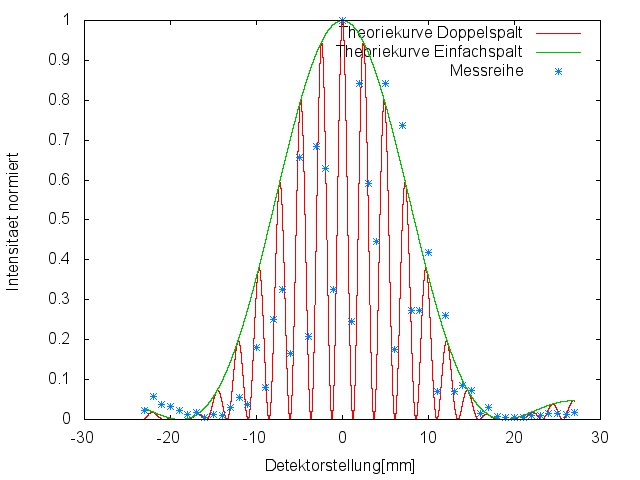
\includegraphics[width = 14cm]{graph3.jpg}
			\caption{Graphische Darstellung der Beugung eines festen Doppelspalts}
			\label{graph3}
		\end{figure}
		\clearpage
